% Source-locked numerical result only: see GitHub Actions 38388066957, 38315269388.
% Exact aligned native EEG payload block census, not inferred clinical identity.
\begin{figure}[tb]
\centering
\begin{minipage}[t]{.50\linewidth}
\centering
\textbf{(a) Published EDF digital EEG block identity}\\[3pt]
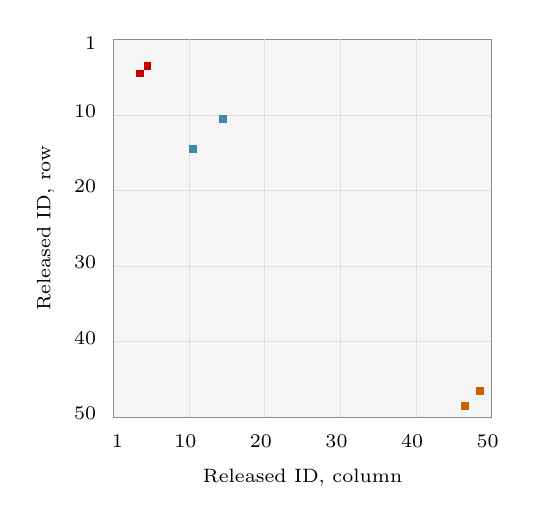
\begin{tikzpicture}[x=0.096cm,y=0.096cm]
\fill[black!4] (0,0) rectangle (50,50);
\draw[black!45,thin] (0,0) rectangle (50,50);
\foreach \i in {10,20,30,40} {
 \draw[black!12,very thin] (\i,0)--(\i,50);
 \draw[black!12,very thin] (0,\i)--(50,\i);
}
% Exact symmetric coordinates:
\fill[red!78!black] (3,45) rectangle (4,46);
\fill[red!78!black] (4,46) rectangle (5,47);
\fill[orange!78!black] (46,1) rectangle (47,2);
\fill[orange!78!black] (48,3) rectangle (49,4);
\fill[cyan!64!black] (10,35) rectangle (11,36);
\fill[cyan!64!black] (14,39) rectangle (15,40);
\foreach \i in {1,10,20,30,40,50} {
 \pgfmathsetmacro{\x}{\i-0.5}
 \node[font=\scriptsize,anchor=north] at (\x,-1) {\i};
 \pgfmathsetmacro{\y}{50.5-\i}
 \node[font=\scriptsize,anchor=east] at (-1,\y) {\i};
}
\node[font=\scriptsize] at (25,-8) {Released ID, column};
\node[font=\scriptsize,rotate=90] at (-9,25) {Released ID, row};
\end{tikzpicture}
\end{minipage}
\hfill
\begin{minipage}[t]{.46\linewidth}
\textbf{(b) Pairwise block fraction}\\[6pt]
{\small
\begin{tabular}{@{}lrr@{}}
\toprule
ID pair & Matches & Fraction\\
\midrule
\textcolor{red!78!black}{4/5} & 9280/9280 & 100.00\%\\
\textcolor{orange!78!black}{47/49} & 6957/9280 & 74.97\%\\
\textcolor{cyan!64!black}{11/15} & 171/9280 & 1.84\%\\
Other 1222 pairs & 0/9280 & 0\\
\bottomrule
\end{tabular}}\\[8pt]
\textbf{(c) Matched refit evaluation}\\[4pt]
{\small
\begin{tabular}{@{}lcc@{}}
\toprule
 & Original $\lambda_A$ & Purged $\lambda_B$\\
\midrule
Nominal fit $F_A$ & .588673 & .587347\\
Content-purged $F_B$ & .580765 & .582551\\
\bottomrule
\end{tabular}}\\[7pt]
{\small\textbf{Interpretation:} Only released digital contents are
fingerprinted. The AUC comparison holds 49 evaluated contents fixed;
it cannot identify patients or a causal population bias.}
\end{minipage}
\caption{Evidence hierarchy for public Liu2024 EEG content overlap.
(a) A sparse symmetric 50-by-50 ID matrix highlighting the three
nonzero aligned-payload cross-ID pairs under the same named channel
and native-record coordinates. (b) Exact equal digital EEG block
counts over 29 time-varying EEG channels and 320 storage records
per file. The remaining 1,222 pairs had no equal aligned payload
blocks; this is not an empirical specificity estimate beyond
the tested release. (c) Descriptive original/purged fit by frozen
source-parameter comparison on 49 held content groups.
The figure is a deterministic visualisation of the archived
public-release measurements, not original clinical provenance.}
\label{fig:p2-native-evidence-matrix}
\end{figure}
